%%%% time
\begin{frame}
\frametitle{Performances - computational time}
\framesubtitle{the exponential kernel in 1D}
\begin{figure}
    \centering
    \begin{subfigure}[b]{0.45\textwidth}
        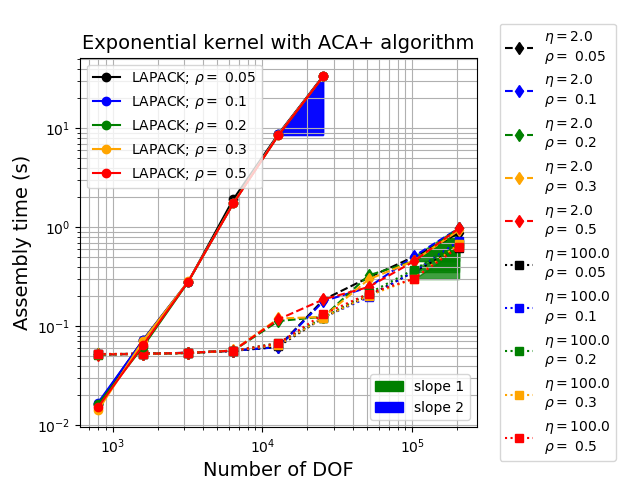
\includegraphics[scale=0.3]{./img/line_EXP_assembly_time}
        \caption{Matrix assembly}
    \end{subfigure}
    \begin{subfigure}[b]{0.45\textwidth}
        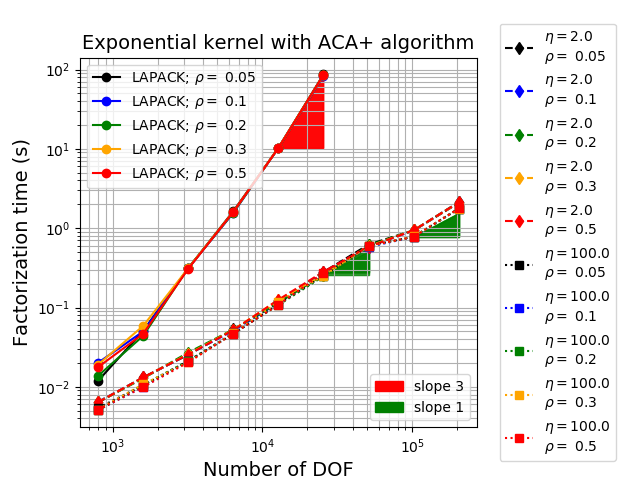
\includegraphics[scale=0.3]{./img/line_EXP_factorization_time}
        \caption{Matrix factorization}
    \end{subfigure}
    \caption{Computational time vs matrix size}
\end{figure}
\end{frame}

%%%% memory
\begin{frame}
\frametitle{Performances - memory}
\framesubtitle{the exponential kernel in 1D}
\begin{figure}
    \centering
    \begin{subfigure}[b]{0.45\textwidth}
        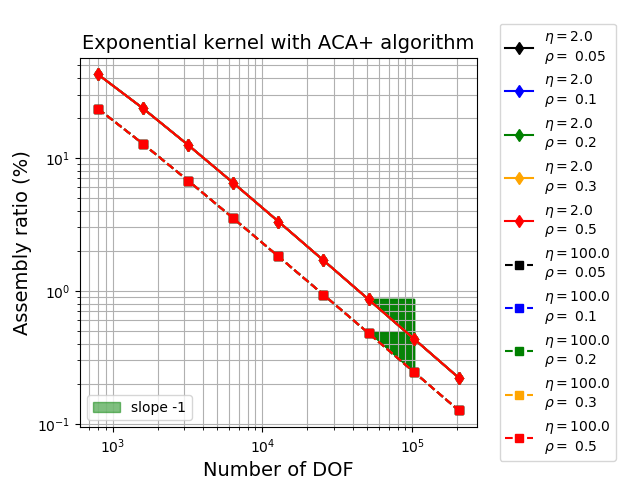
\includegraphics[scale=0.3]{./img/line_EXP_assembly_ratio}
        \caption{Matrix assembly}
    \end{subfigure}
    \begin{subfigure}[b]{0.45\textwidth}
        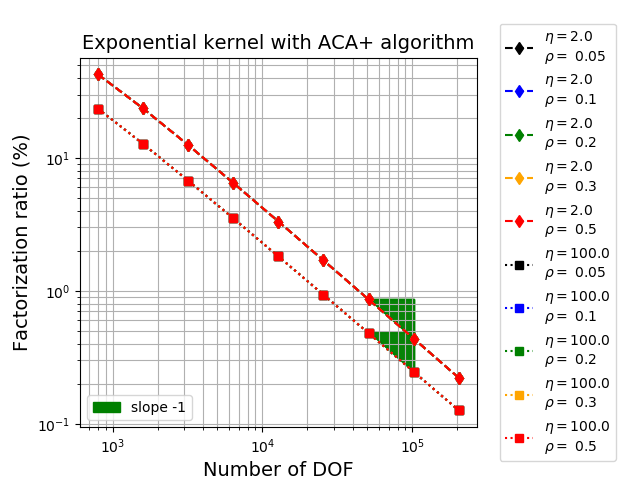
\includegraphics[scale=0.3]{./img/line_EXP_factorization_ratio}
        \caption{Matrix factorization}
    \end{subfigure}
    \caption{Memory vs matrix size}
\end{figure}
\end{frame}
